In this section, we will describe what is the Discrete Fourier Transform (DFT), the Fast Fourier Transform (FFT) and how we use it in our code. First of all, let's consider in all this section two univariate polynomials $f,g \in R[x]$ of degree less than an integer $n$, where $R$ is a commutative ring with units. We want to multiply these two polynomials. To not enter in too much details as we just need to apply the theory, we will consider generally rings such that $R=\mathbb{Z}/m\mathbb{Z}$ with $m\in\mathbb{N}^*$. \\

The product $f\times g$ is of degree less than $2n-1$. We assume we are given a subset $\mathbf{E}$ of $R$ such that $card(\mathbf{E}) = 2n-1$ and that $\forall r \in \mathbf{E}$, we know $f(r)$ and $g(r)$. The values $f(r)g(r)$ can define the polynomial $fg$ completely thanks to the Lagrange interpolation as we have sufficiently values. The cost of defining $fg$ like this is $2n-1$.
To build the coefficients directly of $fg$ has a cost in $\Theta(n^2)$. We want to avoid this high cost using another way to do multiplication : this is what FFT will do. the underlying idea of the fast polynomial multiplication based on the Discrete Fourier Transform is the following : assume that there exists a subset $P$ of $R$ with $2n-1$ elements such that : \\

\begin{itemize}
\item[\textbullet] evaluating $f$ and $g$ at every $r\in P$ can be done at nearly linear time cost, such as $\Theta(n\log(n))$,
\item[\textbullet] interpolating $f(r)g(r)$ for $r\in P$ can be done at nearly linear time cost.
\end{itemize}

Then the multiplication of $f$ by $g$, represented by their coefficients, can be done in $\Theta(n\log(n))$.

\subsection{Discrete Fourier Transform}

\begin{definition*}
Let $n$ be a positive integer and $\omega \in R$. \\
\begin{itemize}
\item[\textbullet] $\omega$ is a $n$-th root of unity if $\omega^{n} = 1$.
\item[\textbullet] $\omega$ is a primitive $n$-th root of unity if :
\begin{itemize}
\item[(1)] $\omega^{n} = 1$.
\item[(2)] $\omega$ is a unit in $R$.
\item[(3)] for every prime divisor $t$ of $n$ the element $\omega^{n/t} - 1$ is neither zero nor a zero divisor.
\end{itemize}
\end{itemize}
\end{definition*}

Let $n$ be a positive integer and $w\in R$ be a primitive $n$-th root of unity. In what follows we identify every univariate polynomial

$$f = \sum_{i=0}^{n-1} f_i\,x^i \in R[x]$$

of degree less than $n$ with its coefficient vector $(f_0,\dots,f_{n-1}) \in R^n$.

\begin{definition*}
The $R$-linear map 

$$DFT_{\omega} : \begin{cases}
R^n &\rightarrow R^n \\
f &\mapsto (f(1), f(\omega), f(\omega^{2}),\dots,f(\omega^{n-1}))
\end{cases}$$
which evaluates a polynomial at the powers of $\omega$ is called the Discrete Fourier Transform (DFT).
\end{definition*}

\begin{proposition*}
The $R$-linear map $DFT_{\omega}$ is an isomorphism.
\end{proposition*}

Then we can represent a polynomial $f$ by the DFT representation with $\omega$ we will determine in our code.

\subsection{Convolution of polynomials}
Let $n$ be a positive integer and $\omega \in R$ be a primitive $n$-th root of unity.\\

\begin{definition*}
The convolution with respect to $n$ of the polynomials $f = \sum_{0\leq i < n} f_i\,x^i$ and $g = \sum_{0\leq i < n} g_i\,x^i$ in $R[x]$ is the polynomial

$$h = \sum_{0\leq k < n}h_k\, x^k$$

such that for every $k \in \mbox{\textlbrackdbl} 0, n-1\mbox{\textrbrackdbl}$ the coefficient $h_k$ is given by

$$h_k = \sum_{i+j\equiv k \mod n}f_i\,g_j$$

The polynomial $h$ is also denoted by $f *_{n} g$ or simply by $f * g$ if not ambiguous.
\end{definition*}

The convolution $f * g$ (of size $n$) and the product $p = fg$ (of size $2n-1$) are different. Let us try to find a relation between these polynomials. We have : \\

$$p = \sum_{k=0}^{2n-2} p_k\,x^k$$

where for every $k \in \mbox{\textlbrackdbl} 0, 2n-2\mbox{\textrbrackdbl}$ the coefficient $p_k$ is given by

$$p_k = \sum_{i+j=k}f_i\,g_j$$

We can rearrange the polynomial $p$ as follows : \\

\begin{align*}
p &= \sum_{0\leq k < n} \left( p_k\,x^k \right) + x^n \, \sum_{0\leq k <n-1} \left( p_{k+n}\,x^k \right) \\
  &= \sum_{0\leq k < n} \left( p_k + p_{k+n}\, (x^n-1+1) \right) \, x^k \\
  &= \sum_{0\leq k < n} \left(\left( p_k + p_{k+n}\, \right) \, x^k \right) + (x^n-1)\, \sum_{0\leq k < n} \left(\left( p_k + p_{k+n}\, \right) \, x^k\right) \\
  &\equiv f * g \mod \left(x^n-1\right) 
\end{align*}


\begin{lemma*}
For $f,g \in R[x]$ univariate polynomials of degree less than $n$ we have 

$$ DFT_{\omega}(f * g) = DFT_{\omega}(f)DFT_{\omega}(g)$$

where the product of the vectors $DFT_{\omega}(f)$ and $DFT_{\omega}(g)$ is computed componentwise.
\end{lemma*}

This lemma allows us to understand that to compute a convolution product is the same as computing a scalar product.


\subsection{The Fast Fourier Transform}

The Fast Fourier Transform computes the DFT quickly and its inverse. This important algorithm for computer science was (re)-discovered by Cooley and Tukey in 1965.\\
Let $n$ be a positive even integer, $\omega \in R$ be a primitive $n$-th root of unity and $f = \sum_{0\leq i<n} f_i\,x^i$. In order to evaluate $f$ at $1, \omega, \omega^{2}, \dots, \omega^{n-1}$, the Cooley-Tukey algorithm follows a divide and conquer strategy. In \cite{FastMulMMM}, Marc Moreno Maza details how this algorithm is done and how the cost of the classical multiplication ($\Theta(n^2)$) can be decreased if we do the multiplication using FFT ($\Theta(n\log(n))$). \\

The picture below shows how we will proceed to multiplicate two polynomials using FFT : \\

\begin{center}
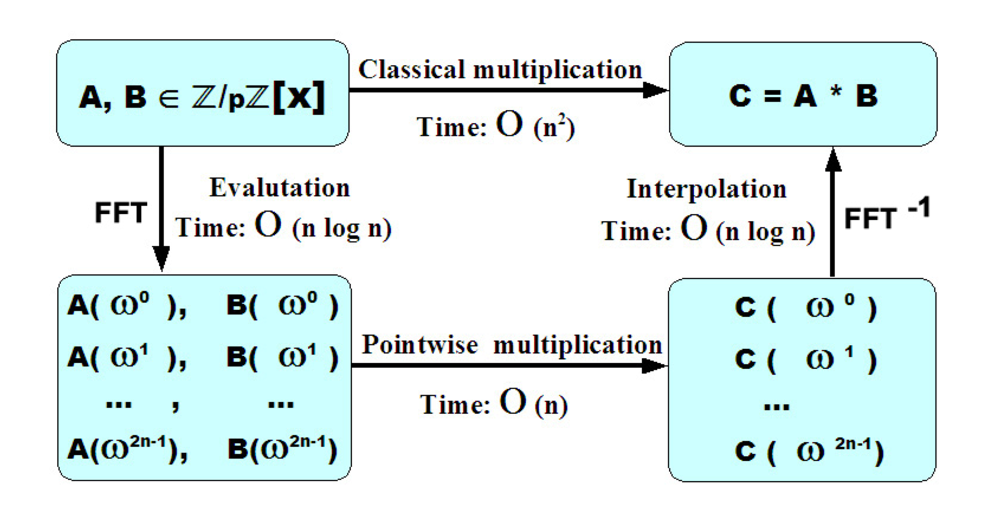
\includegraphics[scale=0.5]{FFT.png}
\textbf{FFT-based univariate polynomial multiplication over $\mathbb{Z}/p\mathbb{Z}$}
\end{center}

